\documentclass[a4paper,10pt,twocolumn]{article}

\usepackage{graphicx}
\usepackage{authblk}
\begin{document}
\title{\emph{BlkKin}: An End-to-end Tracing Tool for Software Defined Storage 
Systems}
\author[1]{Marios-Evangelos Kogias}
\author[1]{Filippos Giannakos}
\author[1]{Vangelis Koukis}
\author[2]{Constantinos Venetsanopoulos}
\author[1]{Nectarios Koziris}
\affil[1]{National Technical University of Athens
Dept. of Electrical and Computer Engineering
Computing Systems Laboratory}
\affil[2]{Greek Research and Technology Network}
\date{}
\maketitle

\section*{Abstract}
Distributed storage systems require special treatment concerning their
monitoring and tracing. BlkKin provides the necessary infrastructure for tracing
software-defined storage systems. It enables live tracing and inserts minimal
overhead to the instrumented system, so that it can continue working effectively
in production scale. Its tracing semantics lead to a cross-layered, end-to-end
representation of the system and how the IO requests interact with it.
End-to-end request tracing enables elaborate information extraction concerning
specific system parts, specific workloads or specific system resources, allowing
the, otherwise impossible, location of latencies and bottlenecks. 
%BlkKin provides a full stack implementation with a data collector, data
%aggregator and a Web UI for visualizing the tracing information can be easily
%incorporated by any system in need of such a tracing framework.

\textbf{Keywords: } tracing, monitoring, low-latency, LTTng, RADOS

\section{Introduction}

The more complex the distributed systems are becoming today, the greater grows
the need for better debugging and monitoring tools. Debugging or monitoring a
distributed system is a difficult and demanding job. Traditional monitoring or
debugging tools like syslog or gdb fail to locate failures or bottlenecks
because dealing with multiple hosts makes the system's behavior unpredictable
and bound to a specific context that could change from execution to execution.

This problem can be tackled through tracing. Tracing captures the state of the
system along with other needed information that could provide further insight
on the exact context in which a specific event happened. The information can be
correlated to explore the system's behavior under different working states.
Unlike traditional monitoring, to obtain this kind of information,
instrumentation points need to be placed in the system's source code indicating
the events to be traced and the values to be measured. Through this
instrumentation we want to trace \textbf{causal relationships} between distinct
software layers, \textbf{latencies} and \textbf{bottlenecks}, as well as
unknown \textbf{execution paths}.

Distributed tracing sets the following challenges. Most of the failures are most
likely to appear at full load. This creates the need for live-tracing under real
working conditions. Ideally we want to have a fully functional system working at
production scale that is getting traced at the same time. Consequently, the
tracing mechanism should not affect the system's performance significantly.
Also, we have to deal with multiple hosts and events happening almost
simultaneously. We need a mechanism that groups scattered but correlated tracing
information and handles with the absence of a global clock.

Some of the most widespread distributed systems are the distributed storage
systems. They can be used either as huge data warehouses for content like images
or videos, or as storage backends for virtual volume provisioning employed by
IaaS providers. In any case, their performance analysis and tuning is of vital
importance for better resource usage and faster, responsive services.

In this paper, we present the design and implementation of \emph{BlkKin}.
BlkKin is a system that enables us to debug and monitor through tracing a
distributed storage system in real time, with very low overhead and visualize
the aggregated information. To build BlkKin we combine various open-source
technologies. We use LTTng (Linux Trace Toolkit - next
generation)\footnote{http://lttng.org/} as tracing backend per host and we
extend it to communicate in real time with
Zipkin\footnote{http://twitter.github.io/zipkin/}, a Twitter's, open-source
implementation of Google's Dapper\cite{dapper}. We created a C/C++ library to
instrument applications according to the semantics described in \cite{dapper}.
Using this library we extended Archipelago\cite{archip} and RADOS\cite{rados} to
support cross-layer tracing, achieving to track any IO request, with an id which
is propagated within the infrastructure, from its creation
till its completion. Apart from the visualization part, this enables us to
extract aggregate time information either per systems' module or per specific
workload.

Related work on the aforementioned problem can be divided into two categories.
There are tools like Ganglia\cite{ganglia} or
ELK\footnote{http://www.elasticsearch.org/overview/} that are more monitoring
oriented. On the other hand, tools like Stardust\cite{stardust} or
Chirp\cite{hp} concentrated mostly on tracing and track capturing and did not
provide live tracing.
 
\section{Background}
In this section we describe why we used Zipkin and LTTng as BlkKin's building
blocks.

\subsection{Tracing logic}
According to \cite{dapper} there are two dominant schools in associating all
record entries with a given initiator. \emph{Black box} monitoring scheme
assumes there is no additional information other than the message record. So
statistical regression techniques should be used to infer any existing
association. \emph{Annotation-based} schemes, though, rely on applications or
middleware to explicitly tag every record with a global identifier that links
these message records back to the originating request. 

For our needed, overall review of the system per specific request, we had to
implement an annotation-based monitoring scheme. In addition, this scheme needs
to depict the causal relationships between the different layers, taking into
account that the system is distributed, thus providing information about the
hosts. Finally, it should enable us to collect any other information considered
important and not restrict us to time data.

Google proposed a complete annotation-based scheme in \cite{dapper}.
This scheme meets the aforementioned demands and is used in
BlkKin. \cite{dapper} describes the following concepts for tracing:

\begin{description}
\item[annotation]
The actual information being logged. There are two kinds of annotations. Either
\emph{timestamp}, where the specific timestamp of an event is being logged or
\emph{key-value}, where a specific key-value pair is being logged.
\item[span]
The basic unit of the process tree. Each specific processing phase can be
depicted as a different span. Each span should have a specific name and a
distinct span id.
\item[trace]
Every span is associated with a specific trace. A different trace id is used to
group data so that all spans associated with the same initial request share the
common trace id. For our case, information concerning a specific IO request
share the same trace id and each distinct IO request initiates a new trace id.
\item[parent span] 
In order to depict the causal relationships between different spans in a single
trace, parent span id is used. Spans without a parent span ids are  known as 
\emph{root spans}.
\end{description}

So, by creating tracing data according to these semantics we can have an
end-to-end sense of our system's performance, behavior and internal latencies
that may vary depending on the nature and size of each request which can also
be captured using key-value annotations.

\subsection{Logic implementation} Based on these primitives, Twitter created
Zipkin, a distributed tracing system used to gather timing data for all the
disparate services running on their premises. Zipkin consists of a data
collector, a database service, with support for a variety of SQL and NoSQL
databases, and a Web interface to visualize the aggregated data.

Zipkin uses Scribe\cite{scribe} to transport traces from the different services
to the central collector. Scribe is a logging server created by Facebook,
aiming to be scalable and reliable.  Scribe servers are arranged in a directed
graph, with each server knowing only about the next server in the graph. This
network topology allows for adding extra layers of fan-in, as a system grows
and batching messages before sending them between datacenters as well as
providing reliability in case of intermittent connectivity or node failure.
Scribe makes use of the Thrift protocol\cite{thrift} for data transfer.

Zipkin seemed to fit our demands concerning data collection since it is
designed to scale. Also, apart from the Web UI, we could execute ad-hoc queries
on the database for more elaborate information extraction, without the need for
batch processing Map-Reduce jobs. However, Zipkin did not provide any C/C++
library to instrument low-overhead applications. The offered libraries were in
scripting languages like Ruby, or in Java and Scala. We created a C/C++ library
that encapsulates the Dapper semantics and can be used within C/C++ projects to
create trace information in accordance with the Dapper logic.  This library is
designed to be backend-independent, which means that one can implement his own
log aggregation backend.  However, we offered a specific backend implementation
according to our initial prerequisites concerning overhead, based on LTTng that
is being thoroughly examined in the next chapter.

\subsection{Tracing Backend}

BlkKin's design was driven by a strict low-overhead and production-wise
operation prerequisite. So the first important decision to make concerned the
system that would implement the system's backend, namely the system that would
run on every cluster node and be responsible for aggregating tracing data from
the instrumented applications. We chose to use LTTng in our system's backend.

LTTng is a toolchain that allows integrated kernel and user-space tracing from
a single user interface. It was initially designed and implemented to
reproduce, under tracing, problems occurring in normal conditions. It uses a
linearly scalable and wait-free RCU (Read-Copy Update) synchronization
mechanism and provides zero-copy data extraction. These mechanisms were
implemented in kernel and then ported to user-space as well. In addition, LTTng
supports a variety of Linux distributions and since version 2.x kernel tracer
modules are built against a vanilla or distribution kernel, without need for
additional patches. The nanosecond-scale added overhead per event traced
mentioned in \cite{desnoyer}, convienced us to use LTTng and have the same
generic toolkit for both user and kernel tracing, wchich can be easily
installed on almost every system needed to instrument. 

Concerning user-space tracing, LTTng supports static tracepoint
instrumentation.  This means to manually insert tracepoints in the application
source code and rebuild the application. After rebuilt, these tracepoints will
get triggered during execution and produce the described traces, without
breakpoints or system-calls. As far a kernel-space is concerned, LTTng is
supported by kprobes\cite{kprobes} and kernel markers\cite{kmarkers}. Thus
LTTng does not significantly affect the system's performance. Although the
whole process of recompiling the instrumented application may seem
counterproductive, static instrumentation abilities are limitless. Based on the
knowledge and understanding of the application, one can instrument and trace
every part that might be problematic or causing longer latencies, as well as
extracting all the information needed to fully understand under which context
each request was served. Consequently, since since we chose to implement the
Dapper tracing semantics, static tracing was the only way to do that.

Finally, live tracing is a prerequisite. Although live monitoring may seem
natural for systems like ELK\footnote, live tracing in combination with
low-overhead was not possible. Older tracing approaches required separation
between the tracing and operation phases. This happened either because tracing
added a lot of extra overhead to the instrumented system so it could not
continue working production-wise, or because tracing information was not in a
state that could be processed before the end of the tracing session. For LTTng
especially, tracing data were in a binary form that could be decoded only after
the end of the tracing session.  However, since version 2.4 of LTTng there is
also live tracing support. Using a daemon called \emph{realyd}, tracing data can
be streamed over TCP forming batch TCP packets and processed while the tracing
session is still in progress. 

\section{Design}
As mentioned, BlkKin was designed respecting four prerequisites:
\textbf{low-overhead tracing}, \textbf{live tracing}, \textbf{Dapper semantics}
and \textbf{Web UI}.

\subsection{BlkKin architecture}
So far we mentioned that we need a tracing agent that run on every host and
captures data produced by the instrumented applications. This agent is LTTng.
Then, data have to be sent in real time to Zipkin. However, LTTng live tracing
supports only CTF\footnote{http://www.efficios.com/ctf} to text
transformations. Consequently, to process and visualize tracing data in real
time in Zipkin, we implemented a live-tracing plugin that transforms in real
time CTF data to Scribe messages and sents them to a Scribe server. Our plugin,
base on Babeltrace\footnote{https://lttng.org/babeltrace}, which is a CTF
converter and trace viewer, reads and decodes the CTF-encoded information,
creates Thrift encoded messages recognizable by the Zipkin collector and sends
these messages to the Scribe server. The plugin is under evaluation for
contribution to LTTng.

So we BlkKin's architecture is presented in Figure\ref{fig:blkin}. The
instrumented application produces tracing information according to the Dapper
semantics using our BlkKin library, through instrumentation points in its source
code. This information is aggregated by LTTng and sent to the relayd. After
that, our Babeltrace plugin gets the tracing data from the relayd, processes
them as mentioned and finally sends them to the Scribe server.

\subsubsection{BlKin Deployment} Each arrow show in Figure ~\ref{fig:blkin}, in
BlkKin's internal architecture represents a TCP communication. Also, the
Scriber server, which the Babeltrace plugin finally sends the tracing
information to, can be either the central Zipkin collector or a local Scribe
daemon that will eventually send the data to the central collector, thus
exploiting the asynchronous, buffered communication provided by Scribe. So we
can have a lot of versatility concerning deployment.

In a cluster deployment with many nodes, we end up having the architecture
presented in Figure~\ref{fig:blkin}. In this deployment, there is a whole
BlkKin stack running on every cluster node. All the communication takes place
over localhost and the tracing data will end up being handled by a local Scribe
daemon. This daemon will normally send the data to the cental Zipkin collector
in batch messages, but also store them locally in case of a connection loss or
if the central Zipkin collector is busy and try to send them later. So through
batch messaging we reduce the Zipkin collector congestion and we can make sure
that no data will be lost, because any data loss would mess up the tracing
semantics and end up with an inconsistent UI and database state.

\begin{figure}[h!]
  \centering
  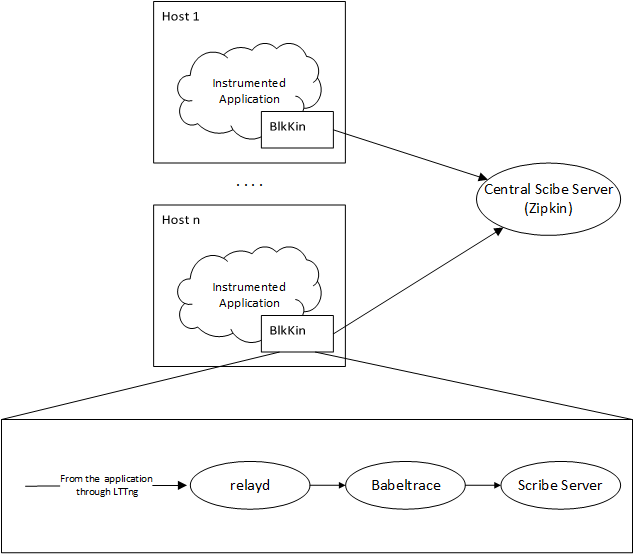
\includegraphics[scale=0.5]{images/blkin2.png}
  \caption{BlkKin deployment and communication}
  \label{fig:blkin}
\end{figure}

\subsection{Clock Synchronization}

A matter that needs special treatment when it comes to distributed
tracing, is clock synchronization. In a BlkKin cluster deployment, ideally we
would like to have no time difference between the clocks of individual cluster
nodes, since we are interested in measuring latencies between nodes and
processing durations in the scale of microseconds. So, a possible time skew in
the scale of milliseconds could result in having a response virtually happening
before its triggering request. The most common solution for clock
synchronization is NTP. Although according to \cite{hp} NTP's accuracy was not
acceptable for tracing, so arithmetic methods had to be deployed to solve the
time skew problem, the NTP v4 published in 2010, improved NTP's potential
accuracy to the tens of microseconds with modern workstations and fast LANs,
through fundamental improvements in the mitigation and discipline algorithms.
So NTP's accuracy fit our needs for clock synchronization.

\section{Implementation} 

Archipelago is a software-defined storage ststem, used in Synnefo\cite{synnefo}
and uses RADOS as a storage backend. Archipelago is structured in a layered
architecture. It offers a QEMU driver for provisioning virtual volumes in
virtual machines. So using our BlkKin library we instrumented the QEMU driver,
Archipelago and RADOS source code. 

\begin{figure}[h!]
  \centering
  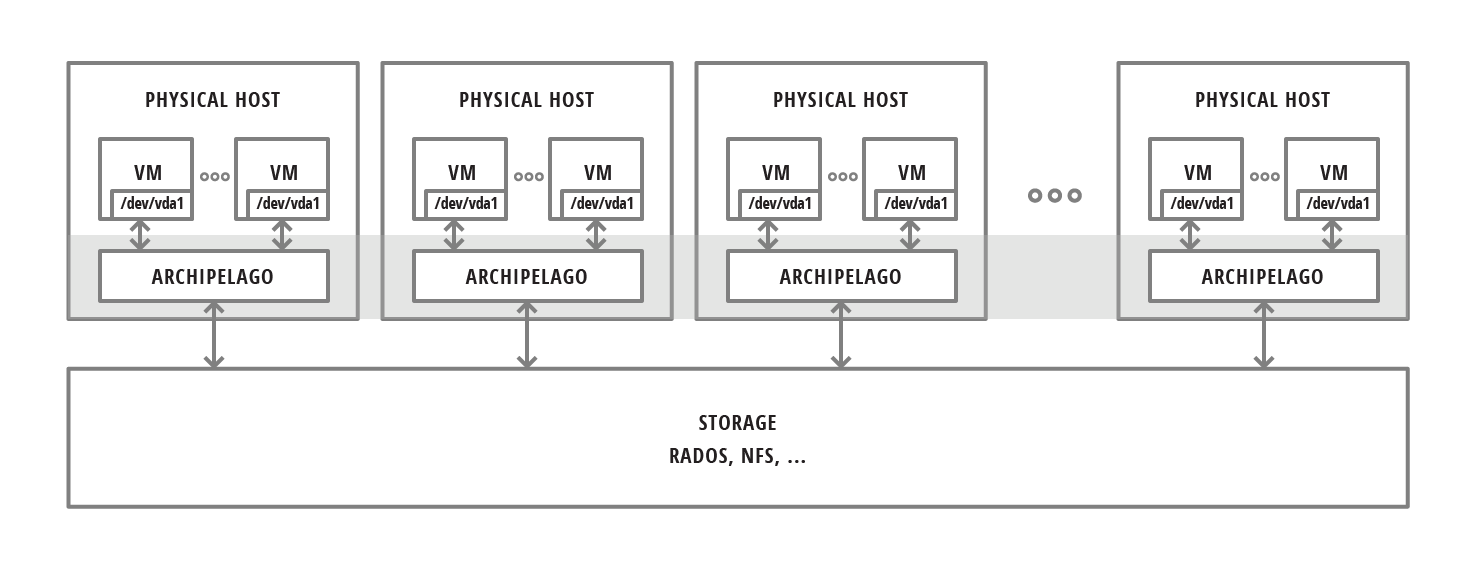
\includegraphics[scale=0.3]{images/archipelago-overview.png}
  \caption{Archipelago overview}
  \label{fig:archipelago}
\end{figure}

Imitating other Zipkin libraries that used HTTP headers to transfer the trace,
span and parent span ids, our library used a struct containing this
information.  This struct is initiated in QEMU and propagated through the
Archipelago layers ,as a separate field in Archipelago requests, and finally
through librados to RADOS. By extending the RADOS internal classes, we managed
to reach this information until the request is served by the filestore.
Overall, we added 113 instrumentation points, that log the separate phases the
IO request passes through and all the needed information concerning the
specific request, like the object name, the request type (read,write) and its
size.

\section{Evaluation - Conclusion} 

We ran benchmarks to evaluate the added overhead that BlkKin poses on
Archipelago and RADOS. For example imitating an IOZone workload we measured the
throughput of 1GB of 64KB sequential writes without instrumentation points and
with instrumentation points with enabled and disabled tracing, since LTTng can
stop the tracing session without affecting the application and start it again if
needed. The results can be seen in the table.

\begin{center}
\begin{tabular}{| l | p{3cm} | p{2cm} |}
    \hline
    Mode & Throughput(MB/s) & Latency/Op (ms)  \\ \hline
    not instrumented & 12.7 & 5.16  \\ \hline
    instrumented stopped & 11.8 &  5.56  \\ \hline
    instrumented & 11 & 5.94  \\ 
    \hline
    \end{tabular}
\end{center}

So, the layered multi-node architecture shown in Figure \ref{fig:archipelago},
after being traced with BlkKin, ends up as shown in Figure \ref{fig:zipkin} in
the Zipkin UI. Each bar represents a distinct processing phase.

\begin{center}
\begin{figure}[h!]
  \centering
  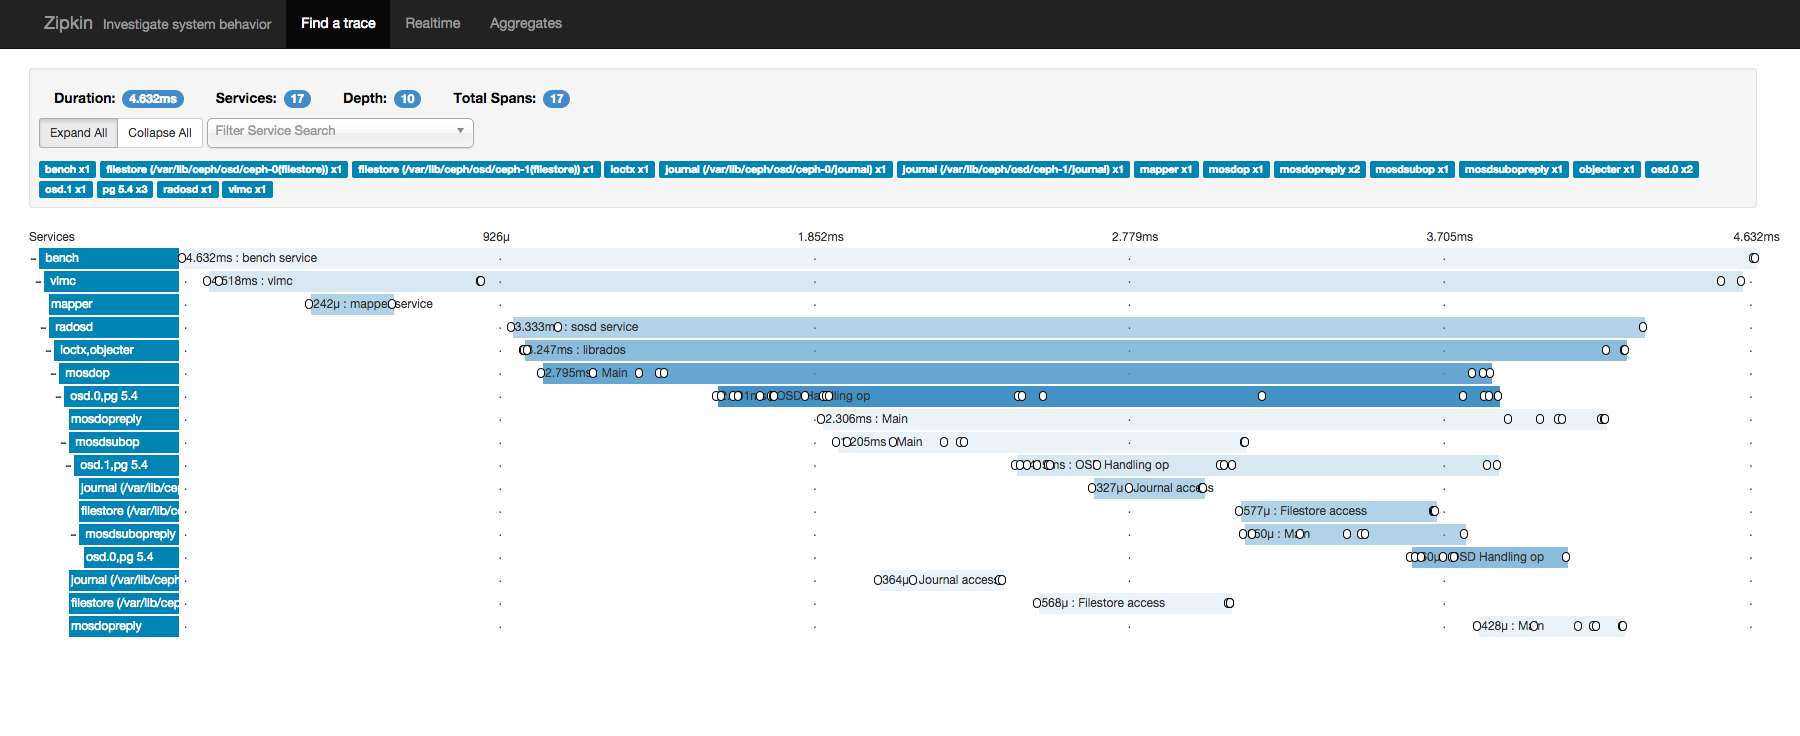
\includegraphics[scale=0.15]{images/zipkin.png}
  \caption{Zipkin UI}
  \label{fig:zipkin}
\end{figure}
\end{center}
Apart from the UI that gave as an overall impression about the systems'
performance and bottlenecks, using simple SQL-queries we were able to calculate
average metrics like each layer's duration, the communication latency between
Archipelago and RADOS or the time that a request stayed in RADOS's dispatch
queue before being served.   

To sum up, we created a working prototype for a low-overhead, live-tracing
infrastructure based on open-source technologies. Using BlkKin we can extract
information not only per system's component but also, per request. Exposing the
system's internals under any possible workload can lead to more reliable
distributed systems.

\bibliography{references}
\bibliographystyle{plain}
\end{document}
